\documentclass[compress]{beamer}
\usepackage{graphicx,amsmath,amsthm,verbatim,bm}
\usepackage{longtable}
\usepackage{booktabs}       % professional-quality tables
\usepackage{tabularx}
\usepackage{multirow}
%\usetheme{Copenhagen}
%\useoutertheme[{options}]{tree}
%\setbeamertemplate{footline}[page number]
%\useoutertheme{infolines} 
%\setbeamertem plate{headlirne}{}
\useinnertheme{circles}
\usepackage{comment}
\setbeamertemplate{footline}[frame number]
%\usepackage{times}
%\usepackage[tbtags]{amsmath}
%\usepackage{amssymb}
\usepackage{amsfonts}
\usepackage{multirow}
%\usepackage{slfortheorems}
\usepackage{epsfig}
\usepackage{graphicx}
%\usepackage[small]{caption}
\usepackage[square]{natbib}
%\newcommand{\newblock}{}
\bibpunct{(}{)}{;}{a}{}{,}
\bibliographystyle{ims}
%\usepackage[letterpaper]{geometry}
\usepackage{color}
\setlength{\parindent}{0pt}
\usepackage{bbding}
\usepackage{longtable, booktabs}
\usepackage{amsfonts}
\usepackage{lipsum}
\usepackage{tikz} 
\usetikzlibrary{arrows, snakes, backgrounds, patterns, matrix, shapes, fit, 
calc, shadows, plotmarks}
\useinnertheme{circles}
\usepackage{tabularx}
\setbeamertemplate{caption}[numbered]

\hypersetup{colorlinks=true,urlcolor=blue,linkbordercolor=red,pdfborderstyle={/S/U/W 1}}

\def\spacingset#1{\renewcommand{\baselinestretch}%
  {#1}\small\normalsize} \spacingset{1}
  
  \newcommand{\dblink}{\texttt{\upshape \lowercase{d-blink}}} % Name of scalable Bayesian ER model

\newcommand{\clusters}{\bm{\kappa}}
\newcommand{\cluster}[1]{\kappa_{#1}}
\newcommand{\sizes}{\bm{\mu}}
\newcommand{\size}[1]{\mu_{#1}}

\newcommand{\edist}{\bm{\gamma}}
\newcommand{\shape}{\eta}
\newcommand{\rate}{s}
\newcommand{\betaA}{u}
\newcommand{\betaB}{v}



\usepackage{tkz-berge}
\usetikzlibrary{fit,shapes}

\usepackage{calc}
\usetikzlibrary{decorations.markings}

\tikzstyle{vertex}=[circle, draw, inner sep=0pt, minimum size=6pt]
\newcommand{\vertex}{\node[vertex]}
\newcounter{Angle}


\usepackage{tabularx}

\let\oldvec\vec
\let\oldcomment\comment
\renewcommand{\comment}[1]{\textcolor{blue}{[#1]}}
\renewcommand\vec{\bm}
\newcommand{\simfn}{\texttt{sim}} % similarity function
\newcommand{\truncsimfn}{\underline{\simfn}} % truncated similarity function
\newcommand{\partfn}{\texttt{PartFn}} % partition function
\newcommand{\distfn}{\texttt{dist}} % distance function
\newcommand{\valset}{\mathcal{V}} % attribute value set
\newcommand{\entset}{\mathcal{E}} % set of records that make up an entity
\newcommand{\partset}{\mathcal{P}} % set of entities that make up a partition
\newcommand{\1}[1]{\mathbb{I}\!\left[#1\right]} % indicator function
\newcommand{\euler}{\mathrm{e}} % Euler's constant
\newcommand{\eber}{\texttt{EBER}} % Name of Bayesian ER model
\newcommand{\secref}[1]{\S\ref{#1}} % Section reference



\usepackage{listings}
\usepackage[ruled,lined]{algorithm2e}
\def\algorithmautorefname{Algorithm}
\SetKwIF{If}{ElseIf}{Else}{if}{then}{else if}{else}{endif}

\usepackage{longtable}



\theoremstyle{plain}
\usepackage{amsfonts}
\usepackage{epsfig}
\usepackage{graphicx}
%\usepackage[small]{caption}

\usepackage{zref-savepos}

\newcounter{restofframe}
\newsavebox{\restofframebox}
\newlength{\mylowermargin}
\setlength{\mylowermargin}{2pt}

\newenvironment{restofframe}{%
    \par%\centering
    \stepcounter{restofframe}%
    \zsavepos{restofframe-\arabic{restofframe}-begin}%
    \begin{lrbox}{\restofframebox}%
}{%
    \end{lrbox}%
    \setkeys{Gin}{keepaspectratio}%
    \raisebox{\dimexpr-\height+\ht\strutbox\relax}[0pt][0pt]{%
    \resizebox*{!}{\dimexpr\zposy{restofframe-\arabic{restofframe}-begin}sp-\zposy{restofframe-\arabic{restofframe}-end}sp-\mylowermargin\relax}%
        {\usebox{\restofframebox}}%
    }%
    \vskip0pt plus 1filll\relax
    \mbox{\zsavepos{restofframe-\arabic{restofframe}-end}}%
    \par
}


\usepackage{tikz}
\usetikzlibrary{arrows}

%\usepackage[usenames,dvipsnames]{xcolor}
\usepackage{tkz-berge}
\usetikzlibrary{fit,shapes}

\usepackage{calc}
\usetikzlibrary{decorations.markings}
%
%\tikzstyle{vertex}=[circle, draw, inner sep=0pt, minimum size=6pt]
%\newcommand{\vertex}{\node[vertex]}
%\newcounter{Angle}



%%%to add in new counter for slides in beamer
\newcommand{\beginbackup}{
   \newcounter{framenumbervorappendix}
   \setcounter{framenumbervorappendix}{\value{framenumber}}
}
\newcommand{\backupend}{
   \addtocounter{framenumbervorappendix}{-\value{framenumber}}
   \addtocounter{framenumber}{\value{framenumbervorappendix}} 
}


\newcommand*\oldmacro{}
\let\oldmacro\insertshortauthor
\renewcommand*\insertshortauthor{
  \leftskip=.3cm
\insertframenumber\,/\,\inserttotalframenumber\hfill\oldmacro}




\excludecomment{notbeamer}
\includecomment{beamer}

\newcommand{\lam}{\mathbf{\Lambda}}	
\newcommand{\bX}{\mathbf{X}}
\newcommand{\bY}{\mathbf{Y}}

\title[An Overview of Entity Resolution]
{An Overview of Entity Resolution}
\author[Rebecca C. Steorts, beka@stat.duke.edu]{Rebecca C. Steorts} 

\institute{\normalsize Department of Statistical Science, affiliated faculty in Computer Science, Biostatistics and Bioinformatics, the information initiative at Duke (iiD) and \\the Social Science Research Institute (SSRI) \\ Duke University and U.S. Census Bureau\\ \vspace*{1em}

This work is supported by NSF CAREER Award 1652431 and the Alfred Sloan Foundation (DRB \#: CBDRB-FY20-309).


}







\begin{document}
\begin{frame}
\titlepage
\end{frame}

%\frame{
%
%List all recent collaborators here. Pictures/list. 
%
%Olivier, Brian, Neil, Ben R, Andee, Brenda, Ziacomo, Fienberg, Rob, Anshu, Beidi, Jerry, Tang, Brunero, Andrea, Ted, Mauricio, Sam, Daniel. Put student's/junior collaborators first. 
%
%}

%\frame{
%
%This is joint work with
%
%\begin{enumerate}
%\item Olivier Binette, PhD Student, Duke University
%\item Brian Kundinger, PhD Student, Duke University
%\item Neil Marchant, Former PhD Student, University of Melbourne
%\item Brenda Betancourt, Former Postdoc, Assist Prof, UF
%\item Andee Kaplan,  Former Postdoc, Assist Prof, CSU
%\item Giacomo Zanella, Former Visiting Scholar, Duke, Assist Prof, Bocconi
%\item Beidi Chen, Former PhD Student, Rice University 
%\end{enumerate
%
%
%}

\frame{
%\frametitle{Motivation} 

\begin{figure}[htbp]
\begin{center}
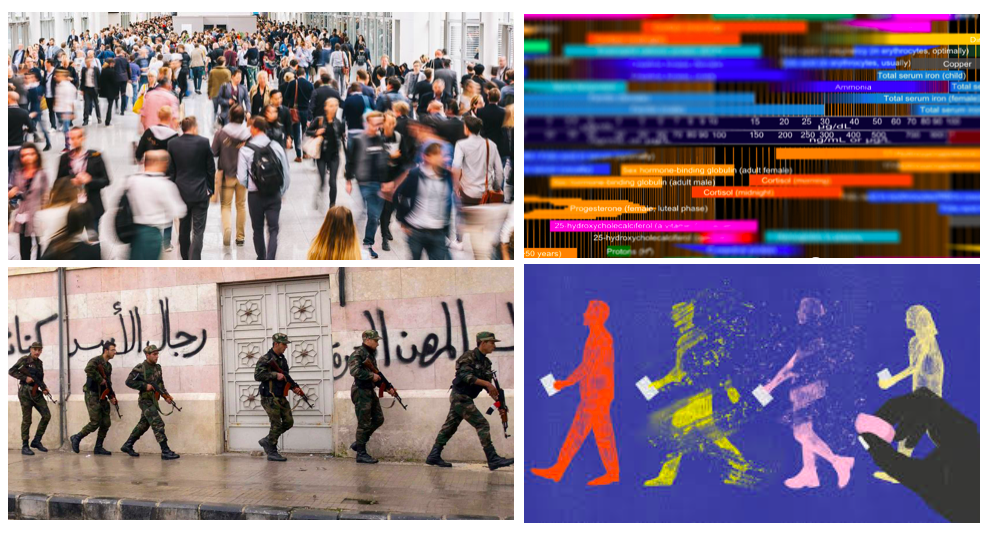
\includegraphics[scale=0.3]{figures/complex-data}

%\caption{default}
%\label{default}
\end{center}
\end{figure}


}

\frame{
\begin{figure}[htbp]
\begin{center}
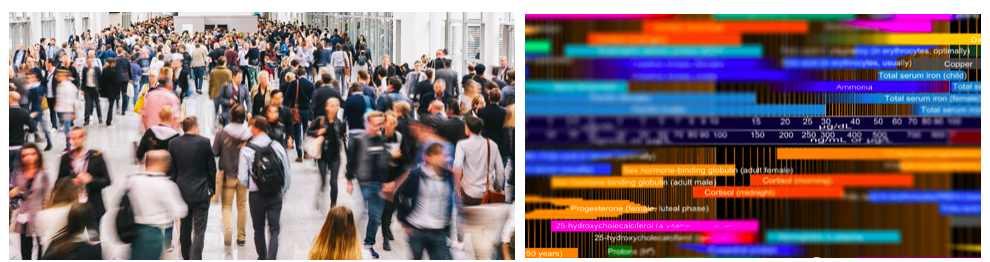
\includegraphics[scale=0.3]{figures/complex-data-top}
%\caption{default}
%\label{default}
\end{center}
\end{figure}

What do these datasets have in common?
\vspace*{1em}
\begin{itemize}
\item There is duplication in the data. 
\item The amount of duplication is typically small. 
\item Before we can apply inferential or prediction methods, any duplicate records must be removed.
\end{itemize}

}

\frame{
\frametitle{Data Cleaning Pipeline}



\begin{figure}[htbp]
\begin{center}
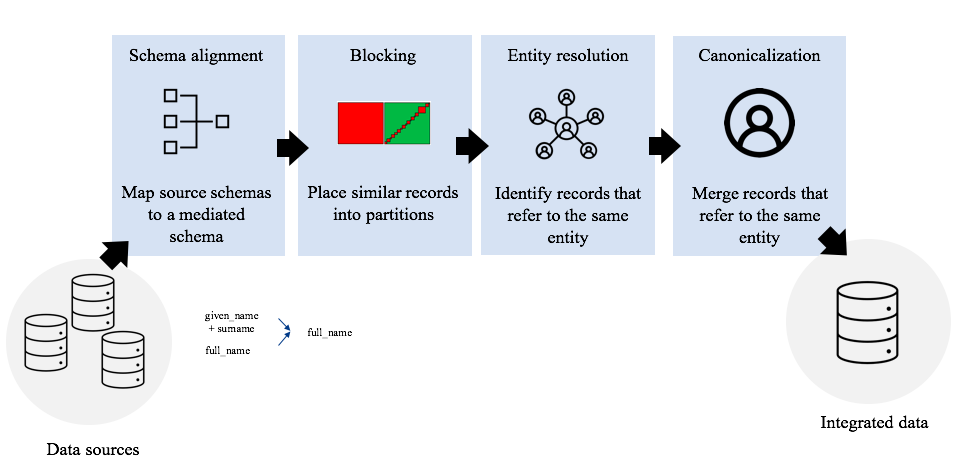
\includegraphics[scale=0.33]{finalFigures/pipeline}
%\caption{default}
%\label{default}
\end{center}
\end{figure}


}

\frame{

\Large
\center

Entity resolution (ER) is the process of merging together noisy (structured) databases to remove duplicate entities, often in the absence of a unique identifier.

}


\frame{

\Large
\center

Other names for entity resolution:  \\

\vspace*{1em}

record linkage, deduplication, duplicate detection, data matching, data integration, data cleansing.

}

%\frame{
%\frametitle{Data Cleaning Pipeline}
%
%
%
%\begin{figure}[htbp]
%\begin{center}
%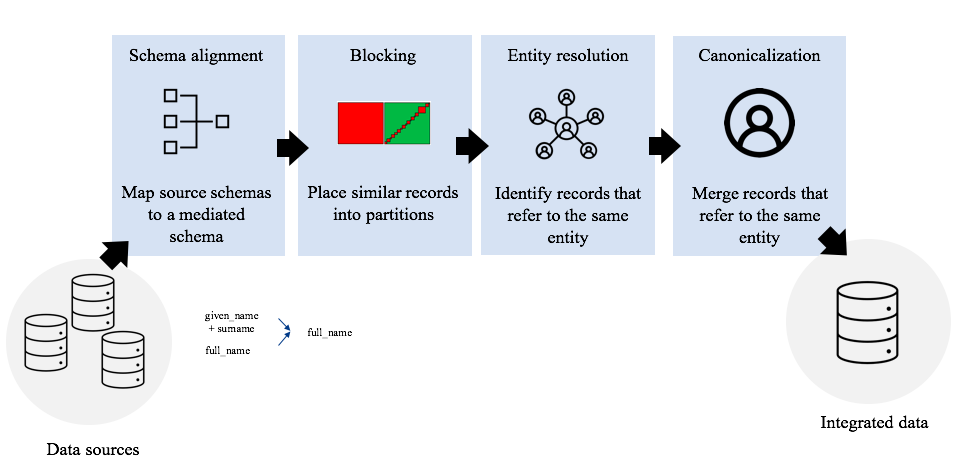
\includegraphics[scale=0.33]{finalFigures/pipeline}
%%\caption{default}
%%\label{default}
%\end{center}
%\end{figure}
%
%\center
%This talk focuses on blocking and entity resolution. 
%
%}

%\frame{
%\begin{figure}[htbp]
%\begin{center}
%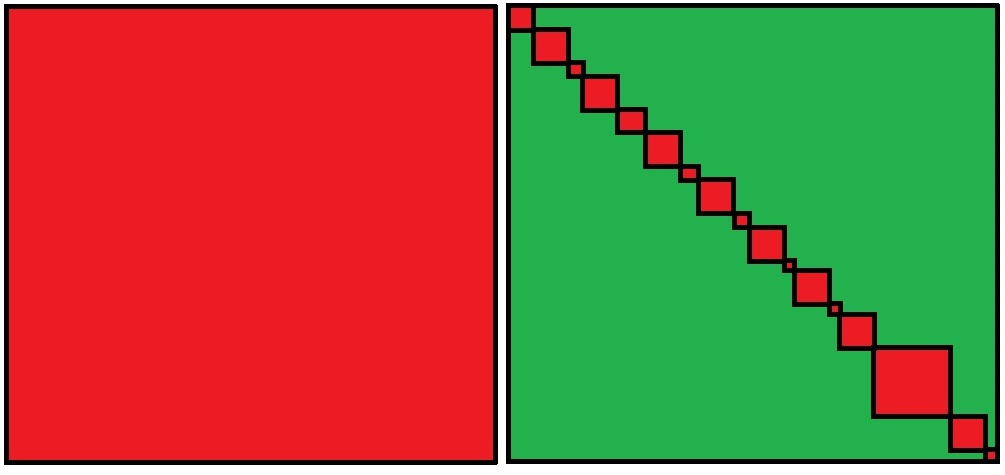
\includegraphics[scale=0.3]{finalFigures/block}
%%\caption{default}
%%\label{default}
%\end{center}
%\end{figure}
%
%\begin{center}
%\Large
%\emph{Blocking is the task of placing similar records into partitions in order to reduce the computational burden of the entity resolution task.}
%\end{center}
%}



%\frame{
%\begin{figure}[htbp]
%\begin{center}
%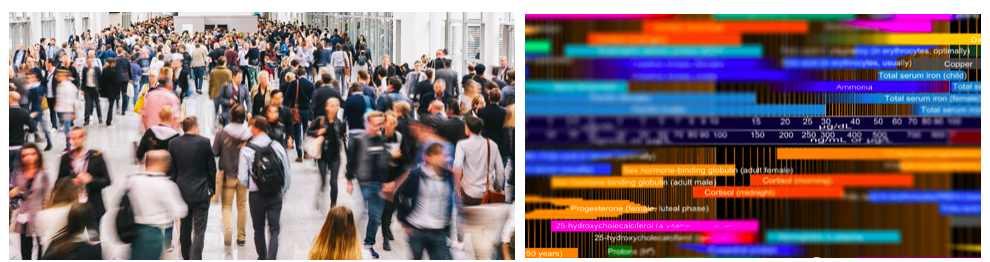
\includegraphics[scale=0.3]{figures/complex-data-top}
%%\caption{default}
%%\label{default}
%\end{center}
%\end{figure}
%
%\begin{center}
%\Large
%\emph{Entity resolution (record linkage or de-duplication) is the task of removing 
%duplicate entities from large noisy data sets, often in the absence of a unique identifier.}
%% (in the absence of a unique identifier). 
%\end{center}
%}

%\frame{
%\frametitle{Recent Work on Blocking}
%
%\begin{enumerate}
%\item Steorts+ (2014) proposed locality sensitive hashing (LSH) methods for blocking and provided comparisons to existing methods in the statistical machine learning literature. 
%\item Sadosky+ (2015) showed that most blocking methods are ill suited for human rights data. 
%\item Shrivastava and Steorts (2018) demonstrated the success of LSH on a case study provided by the Human Rights Data Analysis Group (HRDAG) to the Syrian conflict. 
%\item Edmorado and Steorts (2020) proposed the first approach of the Fellegi and Sunter method for probabilistic blocking that can feed into any entity resolution task. \end{enumerate}
%
%}







\frame{

\begin{center}
\Large
Foundations and Terminology
\end{center}

}

\frame{
\frametitle{A graph with no edges}
\begin{figure}[htbp]
\begin{center}
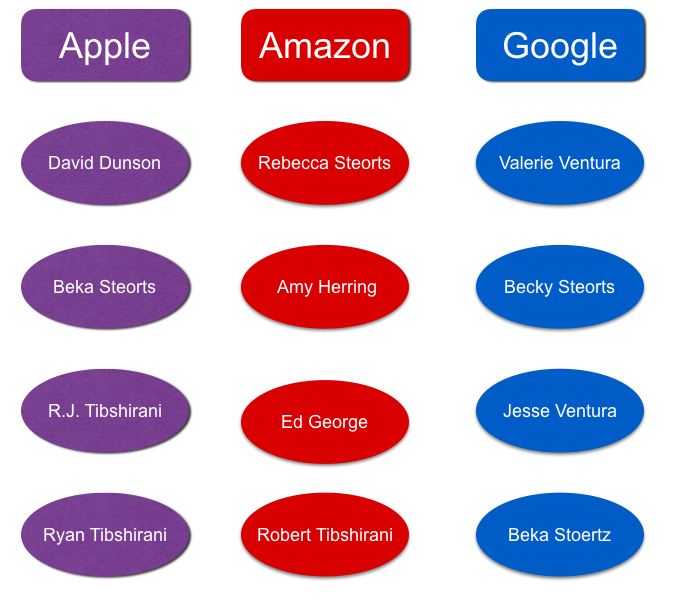
\includegraphics[scale=0.35]{pictures-new/graph-no-edges}
%\caption{default}
%\label{default}
\end{center}
\end{figure}



}

\frame{
\frametitle{The entity resolution graph}
\begin{figure}[htbp]
\begin{center}
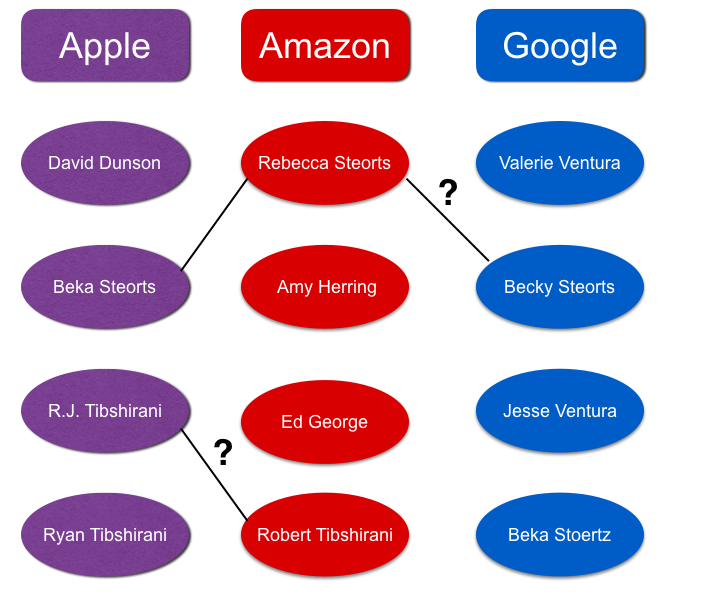
\includegraphics[scale=0.35]{pictures-new/graph}
%\caption{default}
%\label{default}
\end{center}
\end{figure}



}

\frame{
\frametitle{Entities are Real People (Objects, Businesses, Etc.)}
\begin{figure}[htbp]
\begin{center}
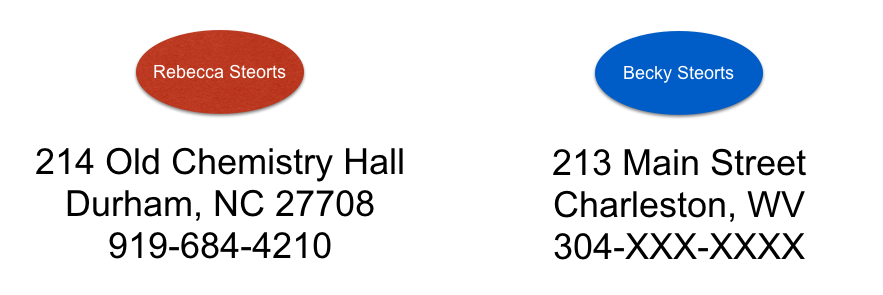
\includegraphics[scale=0.35]{pictures-new/node-two}
%\caption{default}
%\label{default}
\end{center}
\end{figure}



}

%\frame{
%\frametitle{Goal of Entity Resolution}
%
%\begin{figure}[htbp]
%\begin{center}
%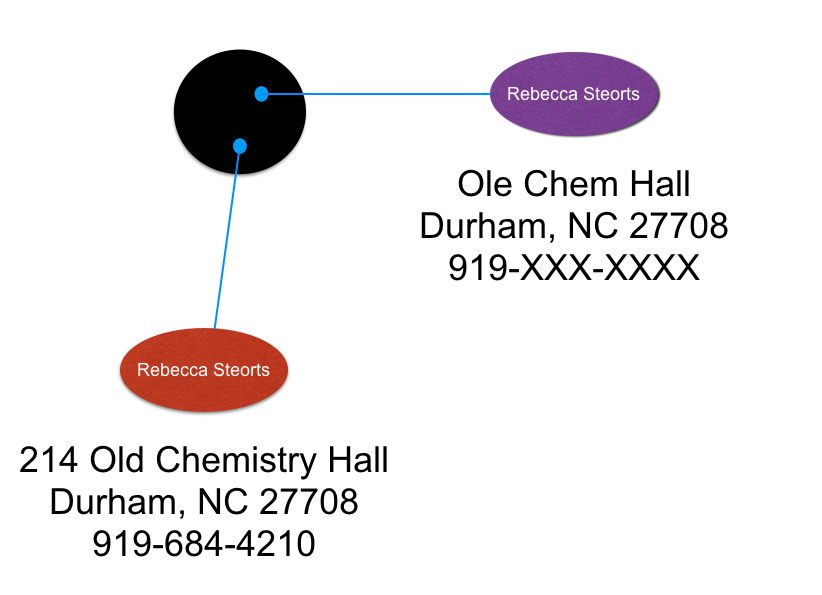
\includegraphics[width=0.6\textwidth]{pictures-new/output-er}
%%\caption{default}
%%\label{default}
%\end{center}
%\end{figure}
%
%%To find the most representative records after ER, one must perform canonicalization (data fusion or merging). 
%
%}

\frame{
\frametitle{Goal of Entity Resolution}

\begin{figure}[htbp]
\begin{center}
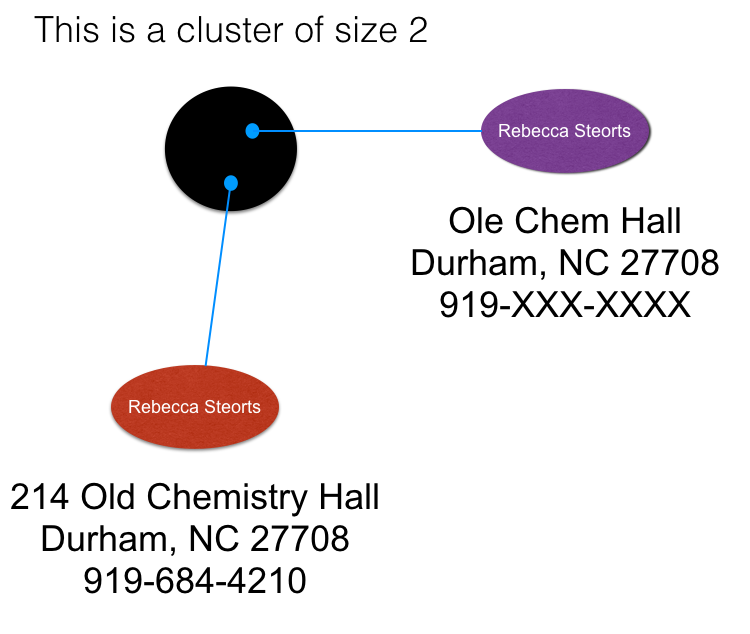
\includegraphics[width=0.6\textwidth]{pictures-new/microcluster}
%\caption{default}
%\label{default}
\end{center}
\end{figure}

%To find the most representative records after ER, one must perform canonicalization (data fusion or merging). 

}

\frame{
\frametitle{Goal of Entity Resolution}

\begin{figure}[htbp]
\begin{center}
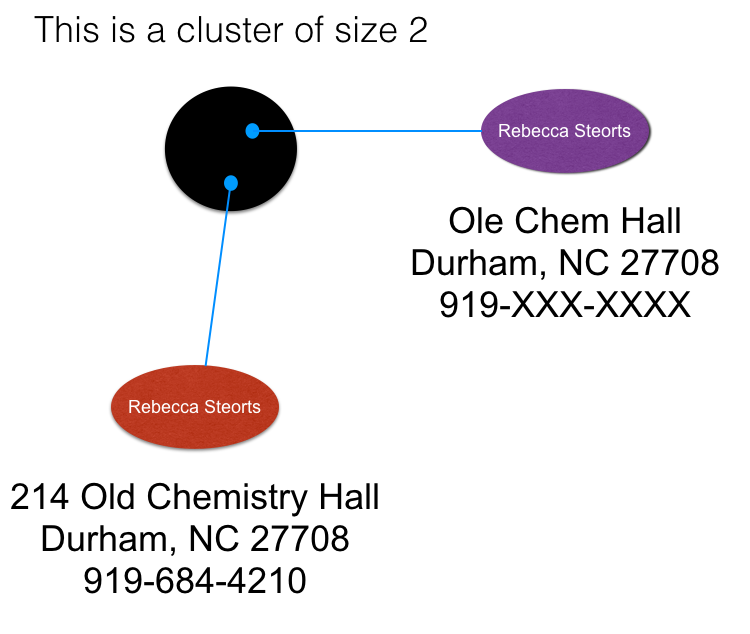
\includegraphics[width=0.6\textwidth]{pictures-new/microcluster}
%\caption{default}
%\label{default}
\end{center}
\end{figure}

To find the most representative records after ER, one must perform canonicalization (data fusion or merging). 

}

\frame{

\Large
\center

In this talk, I will focus on the entity resolution task of the data cleaning pipeline. 

\begin{figure}[htbp]
\begin{center}
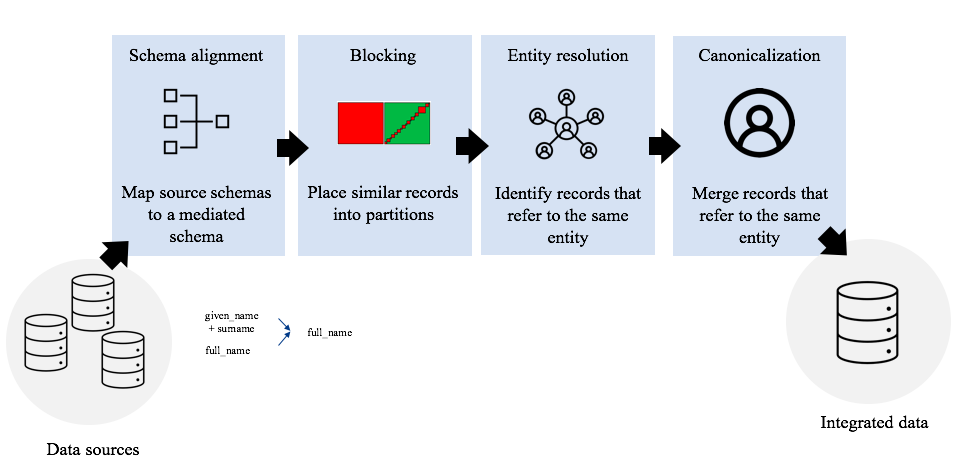
\includegraphics[width=0.9\textwidth]{finalFigures/pipeline}
%\caption{default}
%\label{default}
\end{center}
\end{figure}

%\vspace*{7em}

\normalsize

[Christen (2012), Christophides+ (2021), Papadakis+ (2021), Binette and Steorts (2021)]




}





\frame{
\center
\Large

Challenges

}

\frame{
\frametitle{Challenges of Entity Resolution}

\begin{figure}[htbp]
\begin{center}
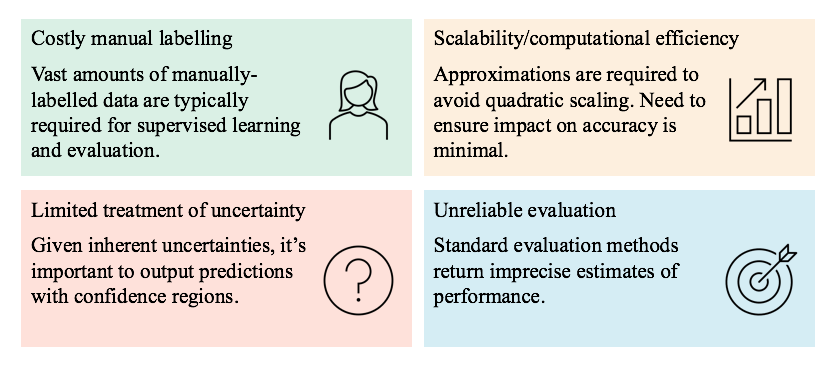
\includegraphics[scale=0.35]{finalFigures/pain-points}
%\caption{default}
%\label{default}
\end{center}
\end{figure}

}




%\frame{
%
%\begin{center}
%\Large
%History
%\end{center}
%
%}

\frame{

\center
\Large
The History of 
Probabilistic Record Linkage

}

\begin{frame}
%{Dunn's ``Book of Life''}
    
\begin{center}
    
\includegraphics[width=0.8\linewidth]{finalFigures/Dunn-0}
\end{center}

\textbf{Halbert L. Dunn} (1896-1975):

\begin{itemize}
    \item Chief of the National Office of Vital Statistics from 1935-1960.
    \item A ``leading figure in establishing a national vital statistics system in the United States".
\end{itemize}

%%The paper ``\textbf{Record Linkage}'':
%%\begin{itemize}
%%    \item adapted from a paper given at the joint conference of the Vital Statistics Council for Canada and for the Dominion Council of Health (Ontario, Canada).
%\end{itemize}
    
\end{frame}

\begin{frame}
%{Dunn's Book of Life}

%\begin{exampleblock}{What this paper does:}

\emph{Record linkage} is the task of assembling together all important pieces of information which refer to the same individual.

%\vspace*{10em}
%
%[Binette and Steorts, 2021 (Major Revision)]

%\vspace*{5em}
%Dunn (1946)
\end{frame}

\begin{frame}
%{Dunn's Book of Life}
    \begin{center}
        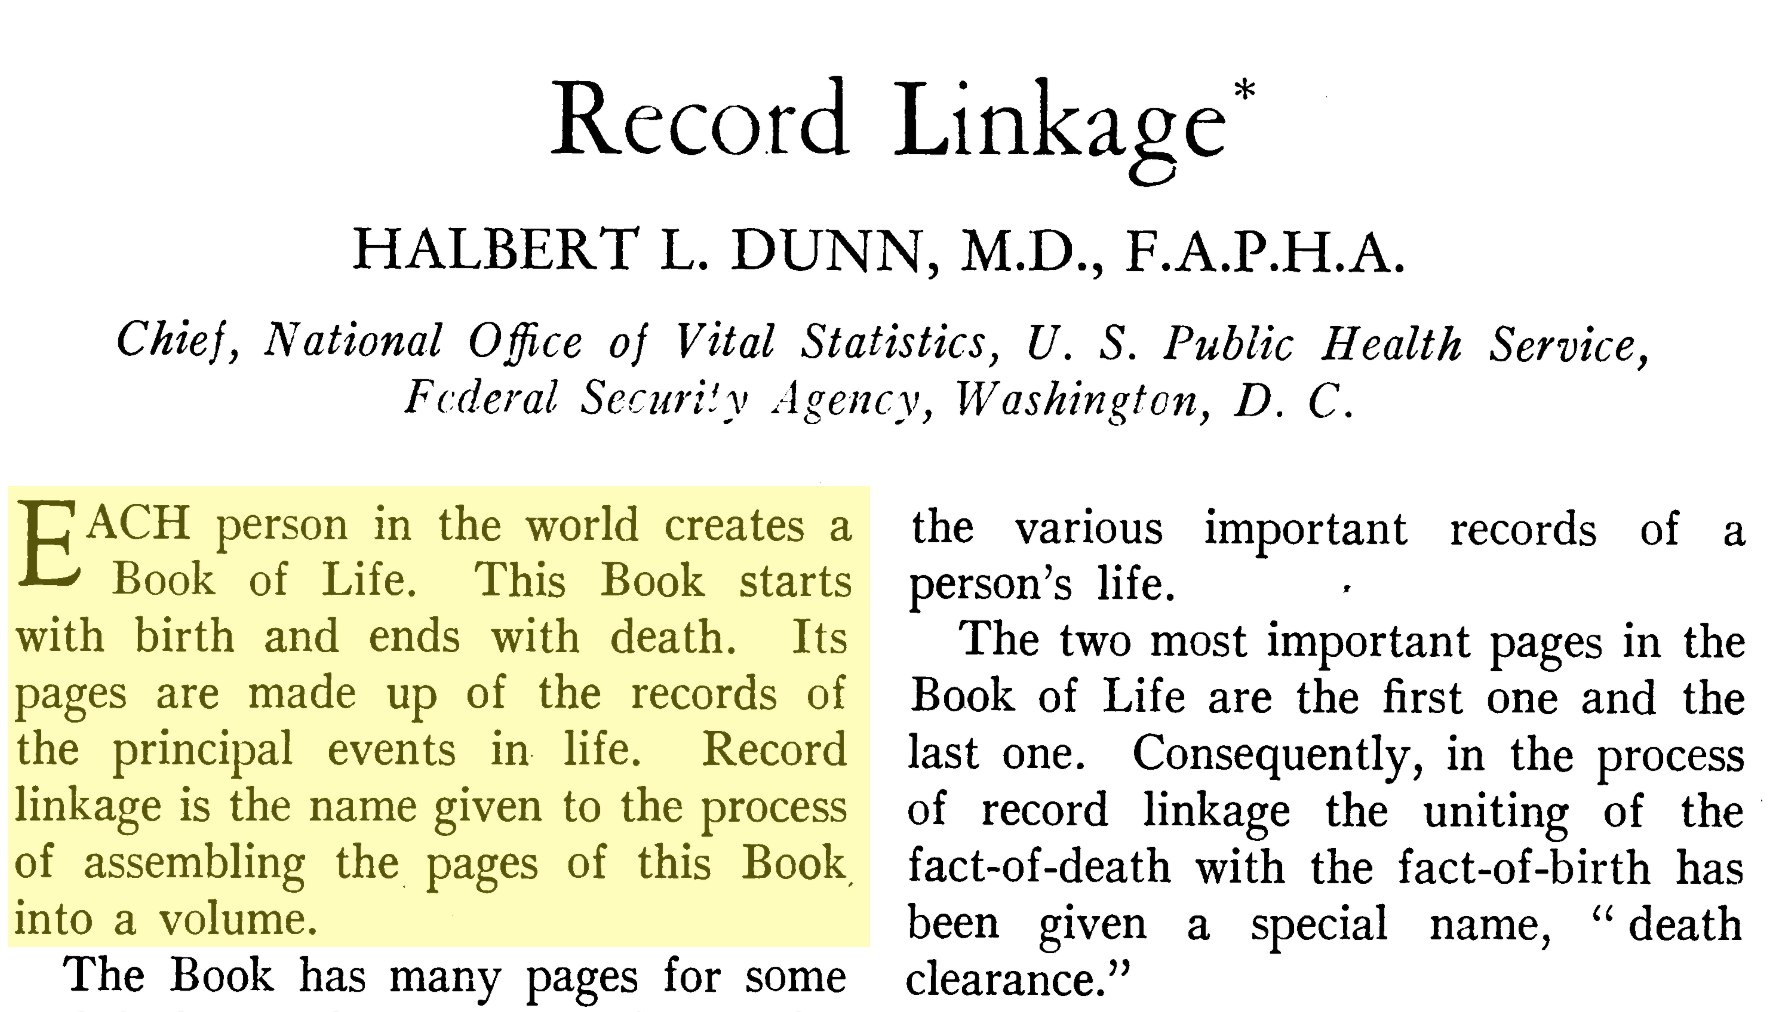
\includegraphics[width=\linewidth]{finalFigures/dunn}
    \end{center}
    

\end{frame}






\begin{frame}
\frametitle{Newcome et al. (1959), Science}
%{Newcombe's computer-based solution}

%Newcombe et al. (1959). Published in \textit{Science}:

\begin{center}
    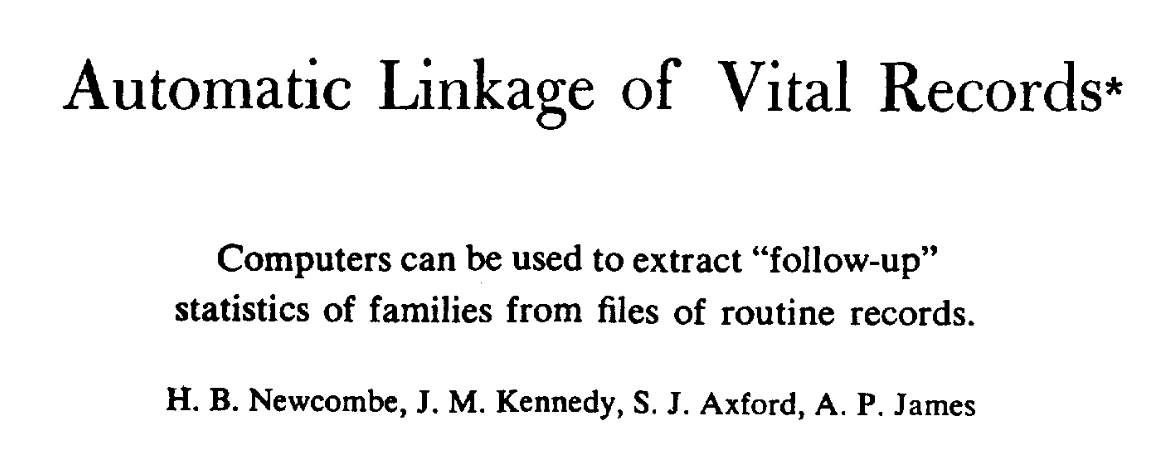
\includegraphics[width=\linewidth]{finalFigures/newcombe}
\end{center}
\end{frame}




\begin{frame}
%{Newcombe's computer-based solution}

Proposed a probabilistic record linkage method and implemented it on the Datatron 205 computer.

\begin{center}
    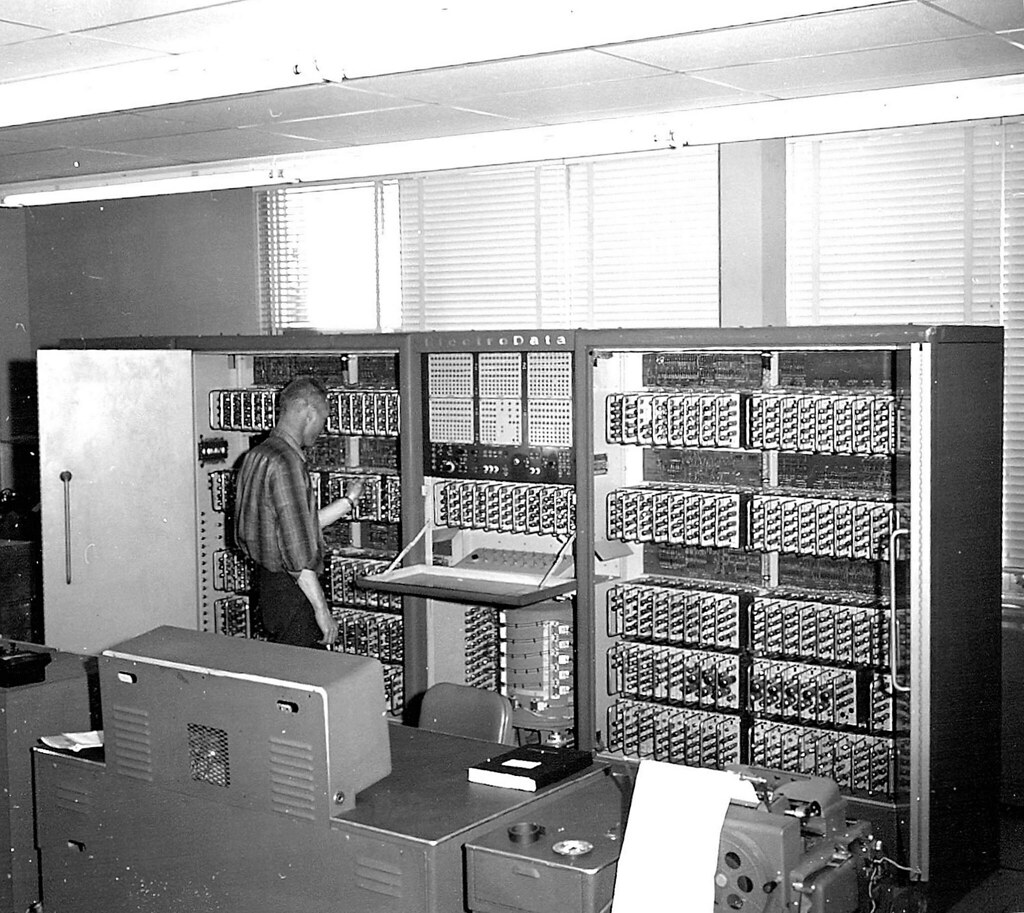
\includegraphics[width=0.6\textwidth]{finalFigures/datatron}
\end{center}

\end{frame}




\begin{frame}
\frametitle{Fellegi and Sunter (1969), JASA}
%{A Theory for Record Linkage}
%Fellegi and Sunter (1969). Published in JASA:
\begin{center}
    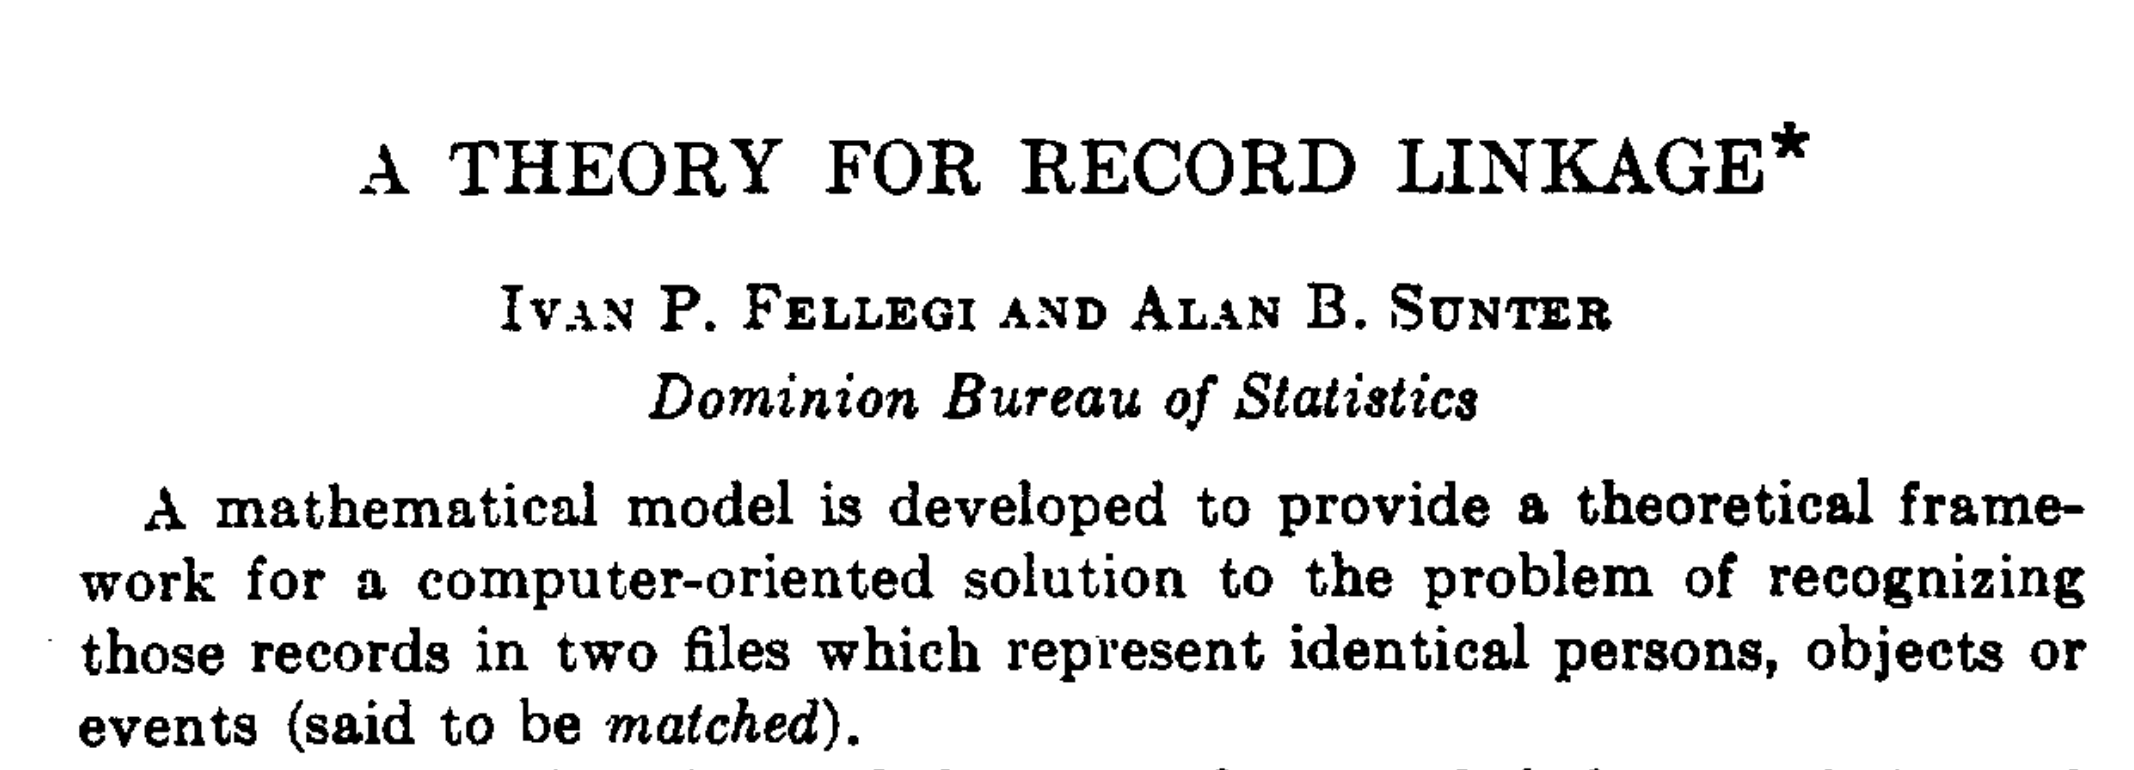
\includegraphics[width=\linewidth]{finalfigures/FS}
\end{center}

\end{frame}




\frame{
\frametitle{Fellegi and Sunter (1969), JASA}

The authors formalized Newcombe et al. (1959) in a decision-theoretic framework. 

\vspace*{1em}

One determines if two records are a match using a likelihood ratio test exceeding a threshold. 

\vspace*{1em}

Many advancements have been made to the original paper, however, I will focus on more modern approaches known as graphical entity resolution that my group has worked on. 


}

\frame{
\center
\Large

Graphical Entity Resolution

}

\frame{
\frametitle{Graphical Bayesian ER}

%\begin{itemize}
%\pause
%\item Dealing with big data means merging large, noisy databases.
%\pause
%\begin{itemize}
%\item Such databases have severe amounts of noise. 
%\end{itemize}
%\pause
%\item Entity resolution requires sophisticated graph structures. [Gutman et. al (2013)].
%\pause
%\begin{itemize}
%\item One approach is to use a bipartite graph for latent entities.
%\pause
%\item Never link records to records. 
%\pause
%\end{itemize}
%\item Computational speed-ups: eliminate low-probability matches.
%%\pause
%%\begin{itemize}
%%\item Blocking techniques based on locality-sensitive hashing.
%\end{itemize}
%\pause
Builds off Copas and Hilton (2001), Tancredi and Liseo (2011).

\begin{figure}[htbp]
\begin{center}
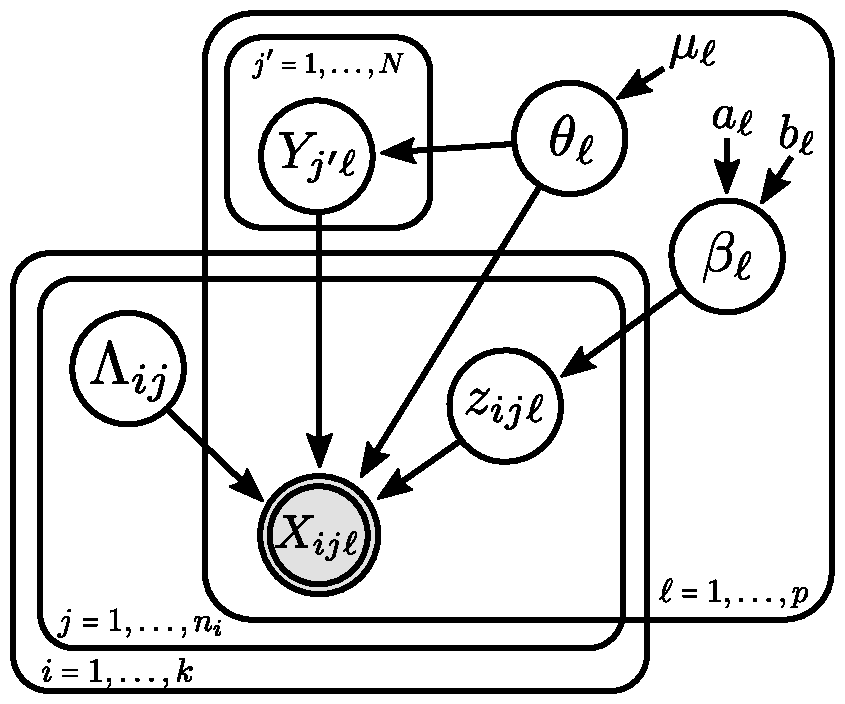
\includegraphics[width=0.5\textwidth]{finalFigures/recordLinkage_graphicalModel}
%\caption{Graphical representation of models \ref{model:cat}-\ref{model:string}.}
\label{fig:graphicalProcess}
\end{center}
\end{figure}

[Steorts+ 2014 AISTATS, Steorts+ 2016 JASA, Steorts 2015 BA]

}

\frame{
\frametitle{Why Graphical Bayesian ER}

\begin{enumerate}
\item Handles any number of databases simultaneously
\item Handles both categorical and textual data
\item Handles missing data 
\item Uncertainty quantification is natural 
\item Transitive closures are nearly free
\item Has sound theoretical properties 
\item Can scale to databases that contain millions of records
\item Generalizes to a wide variety of applications 
\item Has equivalent or better performance than alternatives
\item All software is open source and freely available to non-profits 
\end{enumerate}


}


\frame{

\begin{figure}[htbp]
\begin{center}
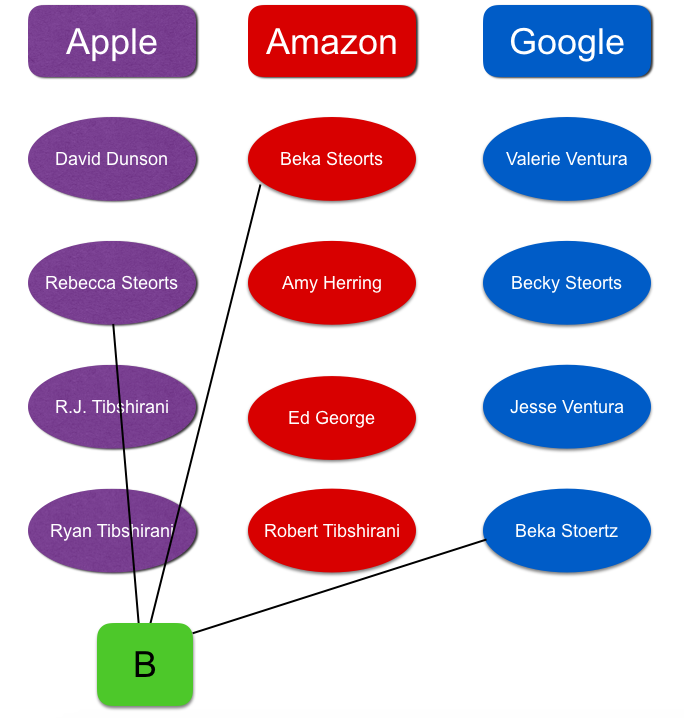
\includegraphics[width=0.7\textwidth]{pictures-new/latent-one}
%\caption{default}
%\label{default}
\end{center}
%\scriptsize{
%\begin{flushright}
%[Steorts, Hall, and Fienberg (2014), \emph{AIStats}.] \newline
%[Steorts, Hall, and Fienberg (2014), \emph{JASA}, In Revision.], [Steorts (2014), Submitted.] 
%\end{flushright}
%}
\end{figure}

}


\frame{

\begin{figure}[htbp]
\begin{center}
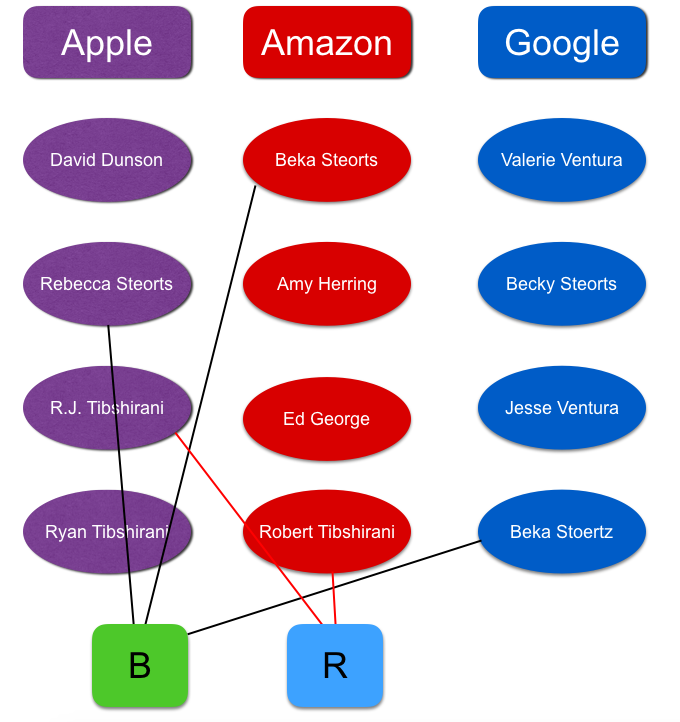
\includegraphics[width=0.7\textwidth]{pictures-new/latent-two}
%\caption{default}
%\label{default}
\end{center}
%\scriptsize{
%\begin{flushright}
%[Steorts, Hall, and Fienberg (2014), \emph{AIStats}.] \newline
%[Steorts, Hall, and Fienberg (2014), \emph{JASA}, In Revision], [Steorts (2014), Submitted.] 
%\end{flushright}
%}
\end{figure}

}



\frame{
\begin{figure}[htbp]
\begin{center}
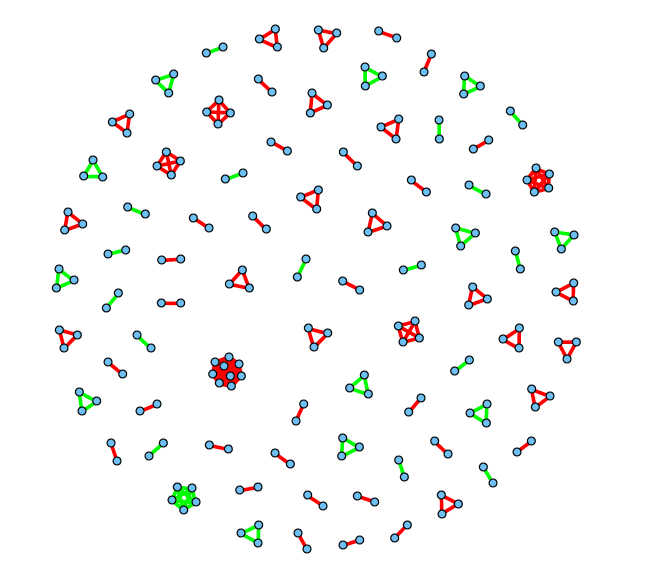
\includegraphics[width=0.7\textwidth]{figures/graph}
\caption{Removing duplications of a longitudinal medical data set (60K). }
%\caption{default}
%\label{default}
\end{center}
\end{figure}
[Steorts+ JASA 2016]

}

\frame{
\begin{figure}[htbp]
\begin{center}
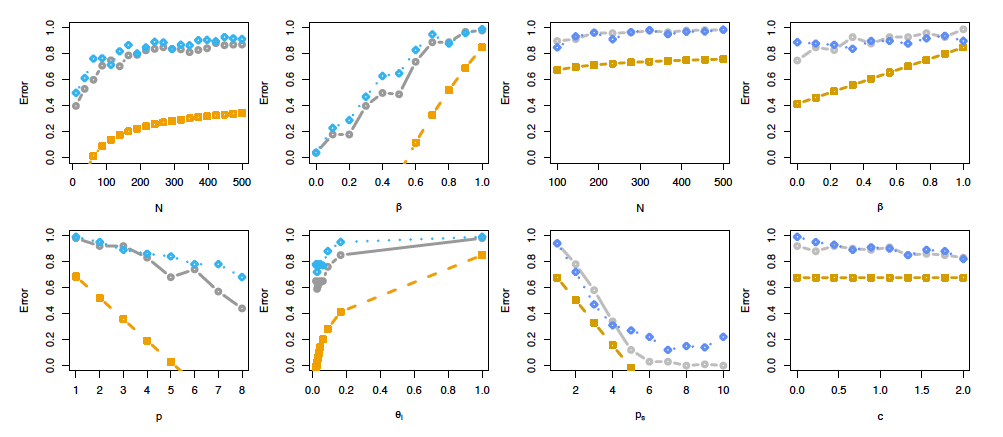
\includegraphics[width=\textwidth]{figures/bounds}
\caption{Bayesian ER models have tight performance bounds.}
%\label{default}
\end{center}
\end{figure}

[Steorts+ AISTATS 2017]

}




\frame{
\frametitle{Our Goal}
\center
\Large

To scale Bayesian ER methods to millions of records without  sacrificing accuracy
   and provide uncertainty of the ER task 

}




\frame{
\center
\Large

We propose a scalable joint (Bayesian) model for blocking and performing entity resolution, where the error from this joint task is measured exactly. 


}





\frame{
\begin{figure}[htbp]
\begin{center}
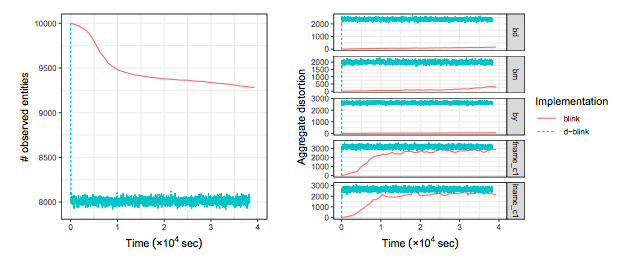
\includegraphics[width=\textwidth]{finalFigures/convergence}
\caption{Comparison of convergence rates for d-blink and blink. The summary statistics for d-blink (number of observed entities on the left and attribute distortions on the right) rapidly converge to equilibrium, while those for blink fail to converge within 11 hours.}
%\caption{default}
%\label{default}
\end{center}
\end{figure}


[Marchant+ (2021) JCGS]
}

\frame{



\scriptsize{
\begin{table}
	\centering
	\caption{Assessment of the pairwise linkage performance for dblink and FS method as our baseline. We note that FS is supervised and does not propagate the entity resolution error exactly compared to dblink.}
	\vspace*{1em}
	\begin{tabular}{l l *{3}{c}}
		\toprule
		Data set    & Method & \multicolumn{3}{c}{Pairwise measure} \\
		\cmidrule(){3-5}
		 & & Precision & Recall & F1-score \\
		\midrule
		\multirow{2}{*}{\texttt{ABSEmployee}} 
		 & dblink                  & \textbf{0.9943} & \textbf{0.8867} & \textbf{0.9374} \\
		 & Fellegi-Sunter (100)  & {0.9964} & {0.9510} & {0.9736} \\
		 & Fellegi-Sunter (10)  & {0.4321} & {0.6034} & {0.9736} \\

		 
%		 & Near matching         & 0.0543 & \textbf{0.9970} & 0.1030 \\
%		 & Exact matching        & \textbf{0.9964} & 0.8849 & 0.9374 \\
		\midrule
		\multirow{2}{*}{\texttt{NCVR}}
		 & dblink                 & \textbf{0.9179} & \textbf{0.9654} & \textbf{0.9411} \\
		 & Fellegi-Sunter (100)  & 0.8989 & {0.9974} & {0.9456} \\
		 & Fellegi-Sunter (10)  & 0.8989 & {0.9974} & {0.9456} \\
%		 & Near matching         & 0.9899 & 0.7443 & 0.8497 \\
%		 & Exact matching        & \textbf{0.9925} & 0.0017 & 0.0034 \\
		\midrule
		\multirow{2}{*}{\texttt{NLTCS}}
		 & dblink                  & \textbf{0.8363} &  \textbf{0.9102} &  \textbf{0.8717} \\
		 & Fellegi-Sunter (100)  & 0.7969 & {0.9959} & {0.8853} \\
		  & Fellegi-Sunter (10)  & 0.1902 & {0.9999} & {0.3196} \\
%		 & Near matching         & 0.0385 & 0.9656 & 0.0740 \\
%		 & Exact matching        & \textbf{0.8451} & 0.9234 & 0.8825 \\ 
		\bottomrule
	\end{tabular}
\end{table}
}
\normalsize
[Marchant+ (2021) JCGS]
}

\frame{
\frametitle{Posterior Bias Plot}

\begin{figure}[htbp]
\begin{center}
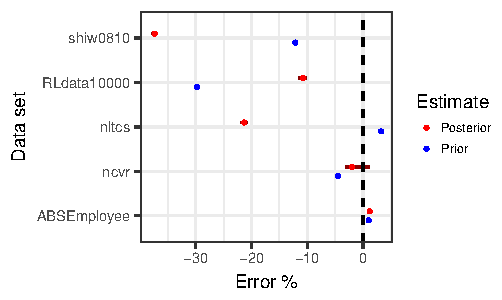
\includegraphics[scale=1]{figures/posterior-bias-plot}
\caption{Error in the posterior and prior estimates for the number of observed entities for d-blink. The results show that the posterior estimate is very sharp and typically underestimates the true number, which is consistent with Steorts, Hall, Fienberg (2016). }
\label{default}
\end{center}
\end{figure}

[Marchant+ (2021) JCGS]

}

\frame{
\frametitle{Case Study Applied to the 2010 Decennial Census}

\begin{table}
  \centering
  \caption{Results for ER of 2010 Census and Numident data in Wyoming. 
  Pairwise evaluation measures are computed using ground truth identifiers 
  available for a subset of the records, where the unadjusted count was reported to be 563,626.}
  \label{tbl:census-results}
  \footnotesize
  \begin{center}
  \begin{tabular}{*{3}{c} *{2}{c}}
    \toprule
    \multicolumn{3}{c}{Pairwise measures} & \multicolumn{2}{c}{Posterior population size} \\
    \cmidrule(lr){1-3} \cmidrule(lr){4-5}
    Precision & Recall & F1-score &    Mean & Std.~error \\
    \midrule
    0.97 &   0.84 &     0.90 & 616,000 & 5,000 \\
    \bottomrule
  \end{tabular}
  \end{center}
\end{table}

\vspace*{4em}

[Marchant+ (2021) JCGS]

}

\frame{
\center
\Large

The Microclustering Property 

}

\frame{
\begin{figure}[htbp]
\begin{center}
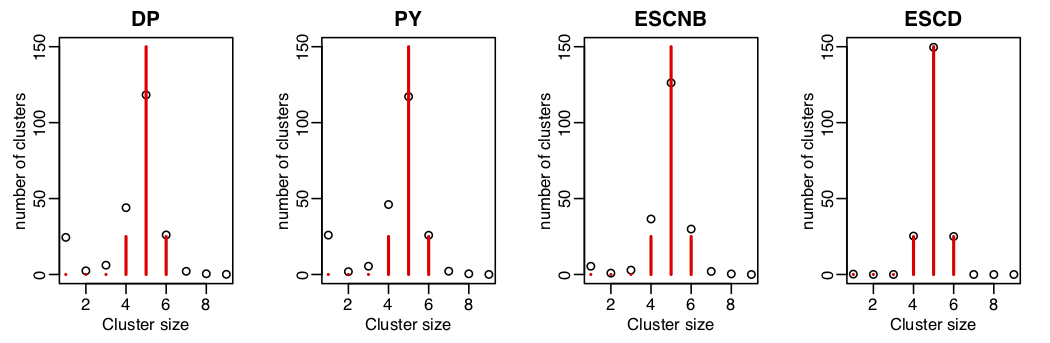
\includegraphics[width=\textwidth]{figures/microclustr}
\caption{Illustrating that infinite dimensional BNPs are often misspecified for ER tasks. }
%\label{default}
\end{center}
\end{figure}
[Zanella+ NIPS 2016, Betancourt+ 2021 JASA]
}





\frame{
\center
\Large

Case Studies Applied to Human Rights Applications

}

\frame{
\begin{figure}[htbp]
\begin{center}
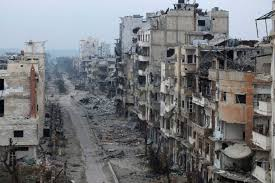
\includegraphics[width=0.7\textwidth]{figures/syria}
\caption{Case study of the number of causalities in Syria (March 2011 -- April 2014) with standard error in real time, matching results of the Human Rights Data Analysis Group (HRDAG).}
%\label{default}
\end{center}
\end{figure}
%[Price+ (2013), Price+ (2015) JRSSA, Sadinle (2014, 2018) AoAS, Chen+ 2018 AoAS]
[Chen+ 2018 AoAS]
}



\frame{
\frametitle{Case Study in El Salvador}

\begin{figure}[htbp]
\begin{center}
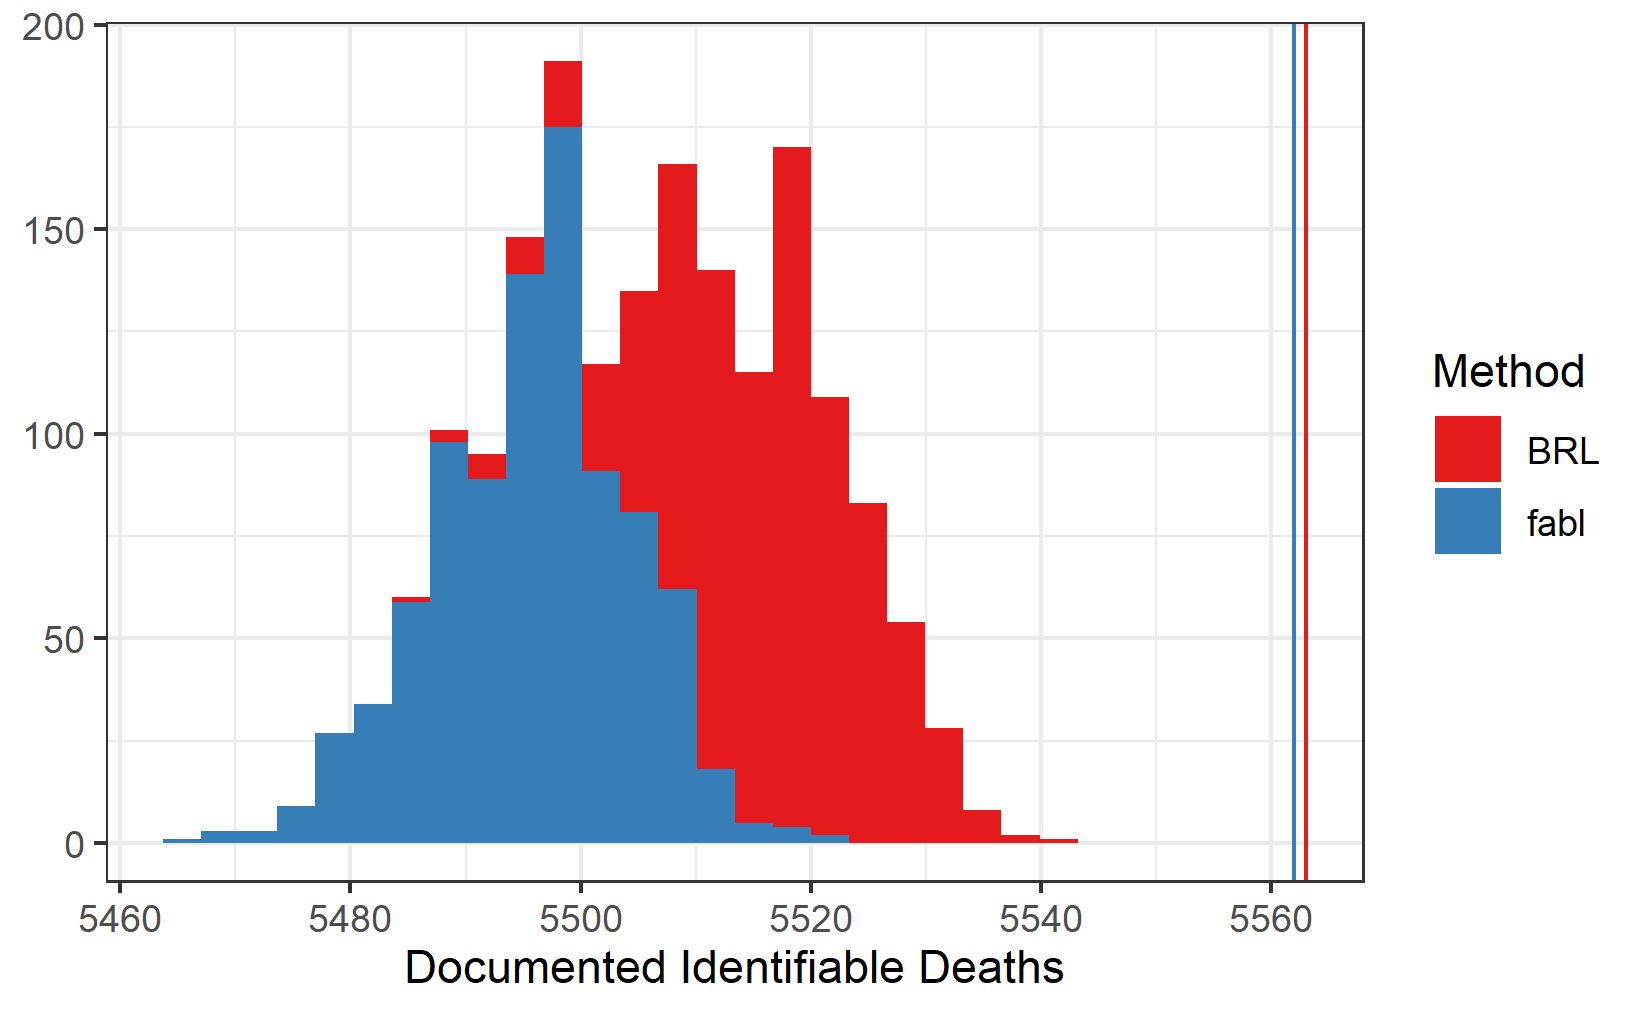
\includegraphics[width=0.8\textwidth]{finalFigures/brian-did-SV}
\caption{Comparison of fabl (our method) compared to Sadinle (2017), known as BRL.}
\label{default}
\end{center}
\end{figure}

[Kundinger, Reiter, Steorts (2021), In Preparation]

}

%\frame{
%\frametitle{Title}
%
%\begin{figure}[htbp]
%\begin{center}
%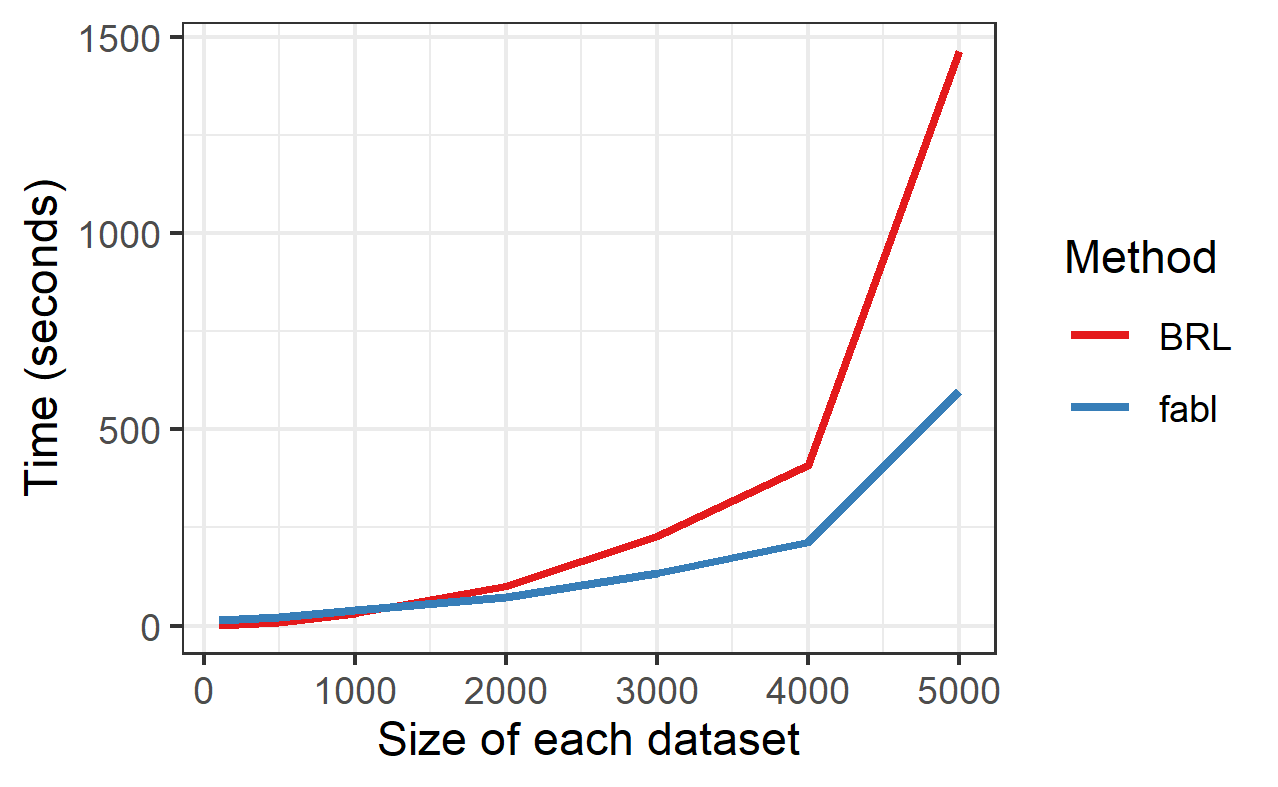
\includegraphics[width=0.8\textwidth]{finalFigures/brian-speed}
%\caption{}
%\label{default}
%\end{center}
%\end{figure}
%
%[Kundinger+ (2021), In Preparation]
%
%}



\frame{
\frametitle{Case study of human trafficking data in the UK}

\begin{figure}[htbp]
\begin{center}
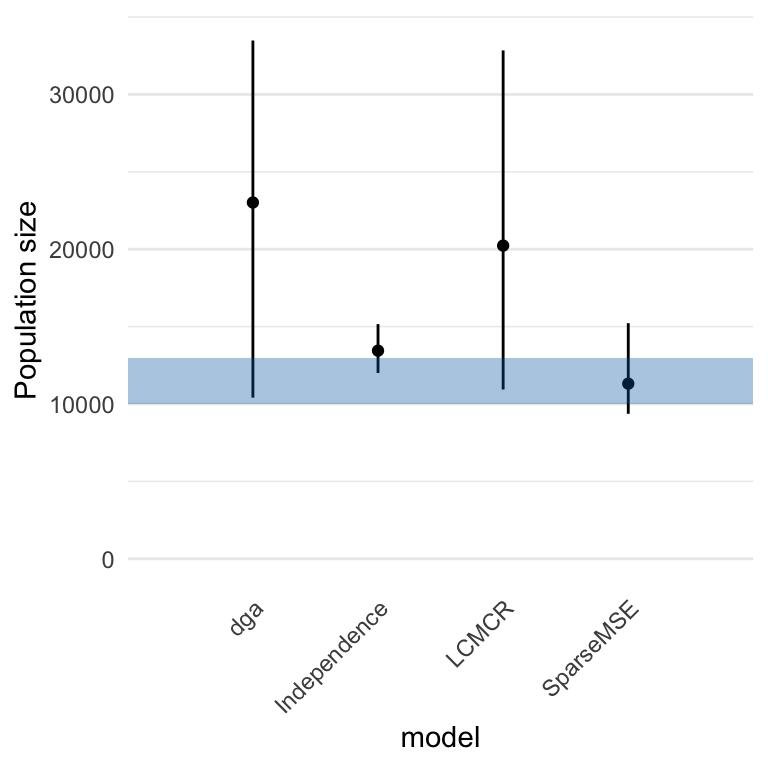
\includegraphics[width=0.6\textwidth]{finalFigures/a_UK_estimates-1}
%\caption{}
\label{default}
\end{center}
\end{figure}

[Binette and Steorts (2021), Submitted]

}

%\frame{
%\frametitle{Title}
%
%\begin{figure}[htbp]
%\begin{center}
%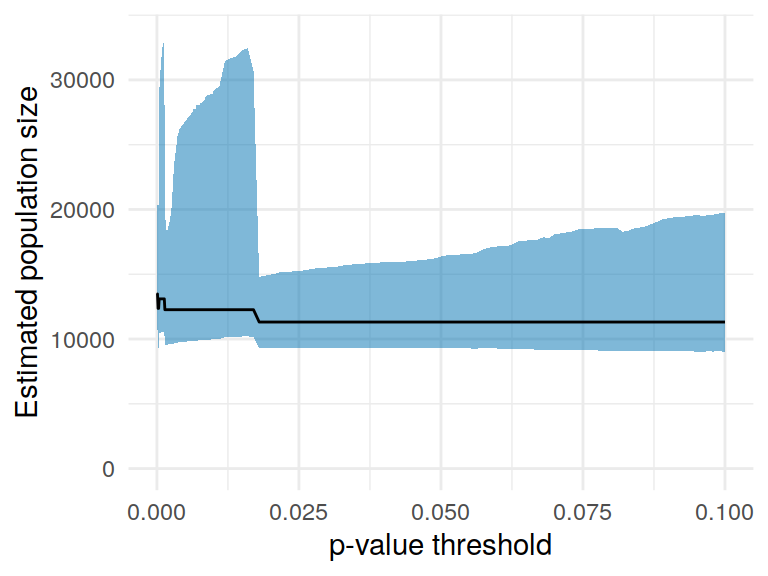
\includegraphics[width=0.8\textwidth]{finalFigures/a_sparsemse_sensitivity_UK-1}
%\caption{}
%\label{default}
%\end{center}
%\end{figure}
%
%[Binette and Steorts (2021), Submitted]
%
%}

%\frame{
%\center
%\Large
%
%Open Questions and Future Directions
%
%}

%\frame{
%\frametitle{Future Directions}
%
%\begin{enumerate}
%\item What benchmark data sets should be used moving forward for entity resolution applications?
%\item Is there one set of agreed upon evaluation metrics that should always be utilized for entity resolution?
%\item What types of evaluation metrics should be used in a fully unsupervised setting?
%\item How do we make sure that entity resolution is used in an ethical way given growing presence of machine learning in daily life?
%\item How can we continue to scale Bayesian methods and push the boundaries of our work to work on larger problems?
%\item What problems do we face regarding hand labelled data and how can we develop methods to evaluate biases or to correct for these?
%
%\end{enumerate}
%
%}

\frame{
\frametitle{This Short Course}

\begin{enumerate}
\item An Overview of Entity Resolution (Just Completed)
\item A Deep Dive Into Entity Resolution
\item Distributed Bayesian Entity Resolution 
\item Distributed Bayesian Entity Resolution with Demos 
\end{enumerate}

\pause
\vspace*{1em}
There are other following materials that may be of interest after completion of this short course: 
\begin{enumerate}
\item \href{https://arxiv.org/abs/2008.04443}{Binette and Steorts Review Article}\\
\item \href{https://github.com/orgs/cleanzr}{Entity Resolution Software}\\
\item \href{https://github.com/cleanzr/record-linkage-tutorial}{Longer Entity Resolution Tutorial}\\
\end{enumerate}

\vspace*{1em}




}




\frame{
\center
Thank you! \\
Questions?\\

\vspace*{2em}
Contact: beka@stat.duke.edu\\
Webpage: resteorts.github.io\\
\vspace*{2em}




}






%\frame{
%
%Add a slide on my joint modeling work with Brunero, Andrea, Jerry, and Tang.
%
%}
%
%
%\frame{
%\begin{figure}[htbp]
%\begin{center}
%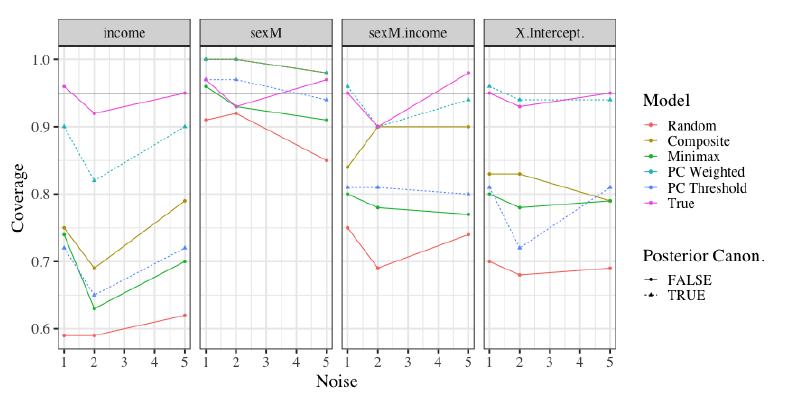
\includegraphics[width=\textwidth]{figures/posterior-canonical}
%\caption{Propagating the ER error into a linear regression task.}
%%\caption{default}
%%\label{default}
%\end{center}
%\end{figure}
%[Kaplan+ (2021), In Revision, TAS]
%%[Steorts+ PSD 2018, Tancredi+ BA 2020, Kaplan+ (2020)]
%}





\end{document}